% Options for packages loaded elsewhere
\PassOptionsToPackage{unicode}{hyperref}
\PassOptionsToPackage{hyphens}{url}
%
\documentclass[
]{article}
\usepackage{amsmath,amssymb}
\usepackage{iftex}
\ifPDFTeX
  \usepackage[T1]{fontenc}
  \usepackage[utf8]{inputenc}
  \usepackage{textcomp} % provide euro and other symbols
\else % if luatex or xetex
  \usepackage{unicode-math} % this also loads fontspec
  \defaultfontfeatures{Scale=MatchLowercase}
  \defaultfontfeatures[\rmfamily]{Ligatures=TeX,Scale=1}
\fi
\usepackage{lmodern}
\ifPDFTeX\else
  % xetex/luatex font selection
\fi
% Use upquote if available, for straight quotes in verbatim environments
\IfFileExists{upquote.sty}{\usepackage{upquote}}{}
\IfFileExists{microtype.sty}{% use microtype if available
  \usepackage[]{microtype}
  \UseMicrotypeSet[protrusion]{basicmath} % disable protrusion for tt fonts
}{}
\makeatletter
\@ifundefined{KOMAClassName}{% if non-KOMA class
  \IfFileExists{parskip.sty}{%
    \usepackage{parskip}
  }{% else
    \setlength{\parindent}{0pt}
    \setlength{\parskip}{6pt plus 2pt minus 1pt}}
}{% if KOMA class
  \KOMAoptions{parskip=half}}
\makeatother
\usepackage{xcolor}
\usepackage[margin=1in]{geometry}
\usepackage{graphicx}
\makeatletter
\def\maxwidth{\ifdim\Gin@nat@width>\linewidth\linewidth\else\Gin@nat@width\fi}
\def\maxheight{\ifdim\Gin@nat@height>\textheight\textheight\else\Gin@nat@height\fi}
\makeatother
% Scale images if necessary, so that they will not overflow the page
% margins by default, and it is still possible to overwrite the defaults
% using explicit options in \includegraphics[width, height, ...]{}
\setkeys{Gin}{width=\maxwidth,height=\maxheight,keepaspectratio}
% Set default figure placement to htbp
\makeatletter
\def\fps@figure{htbp}
\makeatother
\setlength{\emergencystretch}{3em} % prevent overfull lines
\providecommand{\tightlist}{%
  \setlength{\itemsep}{0pt}\setlength{\parskip}{0pt}}
\setcounter{secnumdepth}{-\maxdimen} % remove section numbering
\usepackage[english]{babel}
\usepackage{tcolorbox}
\usepackage{enumitem}
\usepackage{gensymb}
\usepackage{booktabs}
\ifLuaTeX
  \usepackage{selnolig}  % disable illegal ligatures
\fi
\usepackage{bookmark}
\IfFileExists{xurl.sty}{\usepackage{xurl}}{} % add URL line breaks if available
\urlstyle{same}
\hypersetup{
  pdftitle={Description and choice data for the domain ``Sentences''},
  hidelinks,
  pdfcreator={LaTeX via pandoc}}

\title{Description and choice data for the domain ``Sentences''}
\author{}
\date{\vspace{-2.5em}}

\begin{document}
\maketitle

\graphicspath{
  {../experiment/figures/}       % figures used in experiment
}

\subsection{\texorpdfstring{Description of the choice domain 14,
\texttt{Sentences}}{Description of the choice domain 14, Sentences}}\label{description-of-the-choice-domain-14-sentences}

The prompt question and the universe of five response options in the
choice domain \texttt{Sentences} are as follows. The labels \(a\),
\(b\), \(c\), \(d\) and \(e\) were not displayed during the experiment
and are indicated here to allow cross-referencing with data tables and
visualizations below and results in the paper.

\% Sentences

This domain consists of sentences that have been used in experiments of
linguistic judgement. They are, respectively sentences 7j, 7h, 7p, 7a
and 7e in \citeasnoun{BardRobeSora96}. Figure 1 of that paper shows
acceptability scores for these and other sentences given by two
individual linguists, an acceptability score aggregating the scores of
four linguists and an acceptability score aggregating the scores of four
``naive respondents'\,', all undergraduate anatomy students. There is
broad, but not perfect, agreement in terms of order, and in the
following list, they are in decreasing order of acceptability according
to the measure aggregating the judgements of four linguists.

\begin{tcolorbox}
Which one of the following sentences do you find the most grammatically acceptable?

\begin{itemize}
    \setlength\itemsep{-5pt}
    \item Who did Bill buy the car to please?
    \item This is a book which reading would be fun.
    \item Where did Bill buy the car to drive?
    \item Which man do you wonder when to meet?
    \item With which pen do you wonder what to write?
\end{itemize}
\end{tcolorbox}

The following figure is a screenshot from the actual experiment, with
one of the 26 possible menus for this domain.

\begin{figure}
\centering
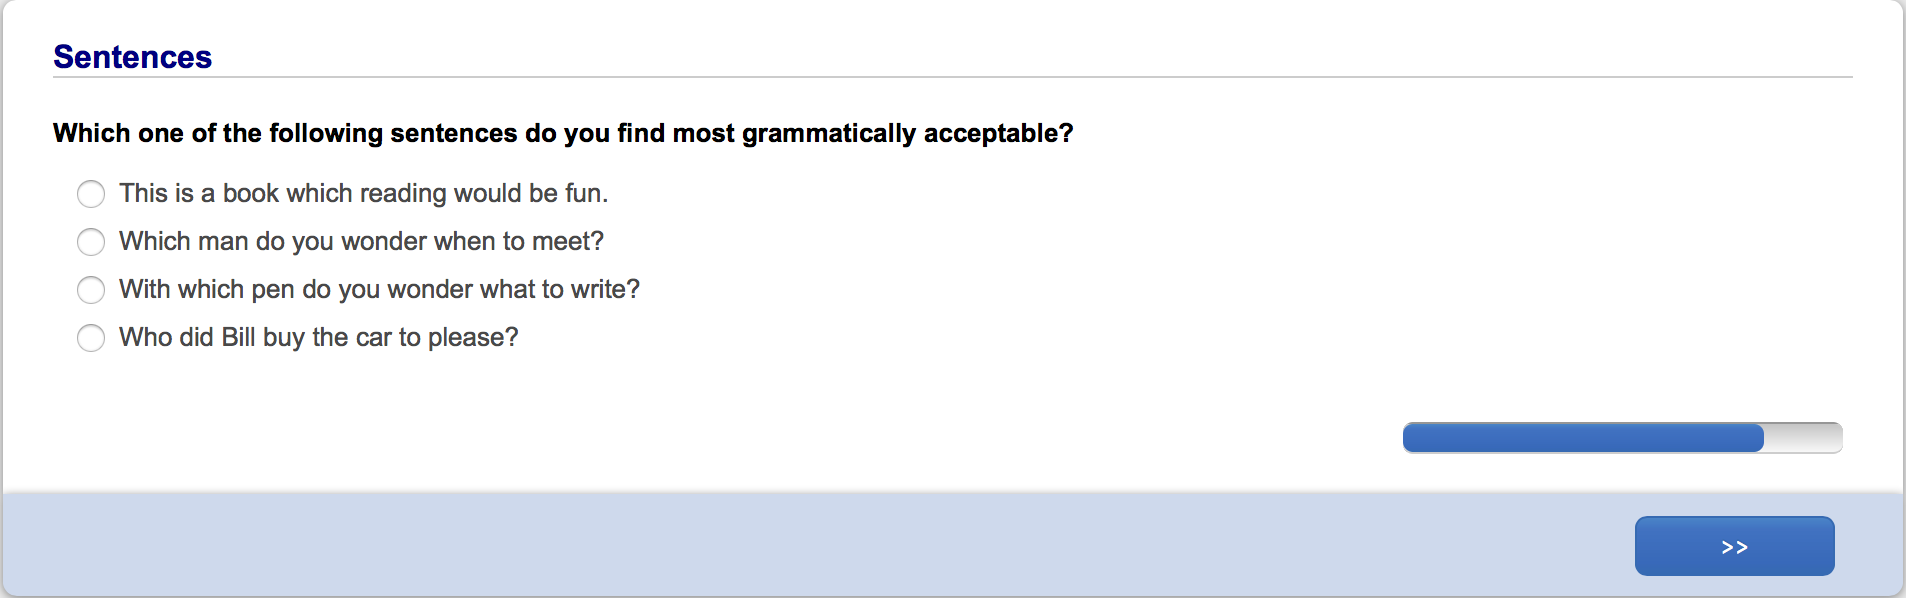
\includegraphics{/Users/williammccausland/Git_repos/Population/experiment/screenshots/screenshot_sentences.png}
\caption{Screenshot for domain Sentences}
\end{figure}

\pagebreak

\subsection{Choice data for domain 14,
Sentences}\label{choice-data-for-domain-14-sentences}

Table \ref{t:count_prop} shows choice counts and choice proportions for
this choice domain. For each menu \(A\) and each object
\(x \in \{a,b,c,d,e\}\), \(N_A(x)\) is the number of participants who
chose object \(x\) from menu \(A\) and \(\hat P_A(x)\) is the
corresponding proportion of participants who chose \(x\) from \(A\).
When \(x \notin A\), a dash is displayed.

\begin{table}\centering

\begin{tabular}{lrrrrrrrrrr}
\toprule
\multicolumn{1}{c}{ } & \multicolumn{5}{c}{Choice counts} & \multicolumn{5}{c}{Choice proportions} \\
\cmidrule(l{3pt}r{3pt}){2-6} \cmidrule(l{3pt}r{3pt}){7-11}
Menu $A$ & $N_A(a)$ & $N_A(b)$ & $N_A(c)$ & $N_A(d)$ & $N_A(e)$ & $\hat P_A(a)$ & $\hat P_A(b)$ & $\hat P_A(c)$ & $\hat P_A(d)$ & $\hat P_A(e)$\\
\midrule
$\{a,b\}$ & 22 & 19 & - & - & - & 0.537 & 0.463 & - & - & -\\
$\{a,c\}$ & 13 & - & 27 & - & - & 0.325 & - & 0.675 & - & -\\
$\{b,c\}$ & - & 16 & 24 & - & - & - & 0.400 & 0.600 & - & -\\
$\{a,b,c\}$ & 20 & 3 & 17 & - & - & 0.500 & 0.075 & 0.425 & - & -\\
$\{a,d\}$ & 28 & - & - & 13 & - & 0.683 & - & - & 0.317 & -\\
\addlinespace
$\{b,d\}$ & - & 30 & - & 10 & - & - & 0.750 & - & 0.250 & -\\
$\{a,b,d\}$ & 21 & 15 & - & 4 & - & 0.525 & 0.375 & - & 0.100 & -\\
$\{c,d\}$ & - & - & 30 & 10 & - & - & - & 0.750 & 0.250 & -\\
$\{a,c,d\}$ & 16 & - & 19 & 5 & - & 0.400 & - & 0.475 & 0.125 & -\\
$\{b,c,d\}$ & - & 12 & 22 & 6 & - & - & 0.300 & 0.550 & 0.150 & -\\
\addlinespace
$\{a,b,c,d\}$ & 10 & 8 & 18 & 4 & - & 0.250 & 0.200 & 0.450 & 0.100 & -\\
$\{a,e\}$ & 19 & - & - & - & 21 & 0.475 & - & - & - & 0.525\\
$\{b,e\}$ & - & 19 & - & - & 21 & - & 0.475 & - & - & 0.525\\
$\{a,b,e\}$ & 17 & 12 & - & - & 11 & 0.425 & 0.300 & - & - & 0.275\\
$\{c,e\}$ & - & - & 26 & - & 14 & - & - & 0.650 & - & 0.350\\
\addlinespace
$\{a,c,e\}$ & 11 & - & 17 & - & 12 & 0.275 & - & 0.425 & - & 0.300\\
$\{b,c,e\}$ & - & 8 & 24 & - & 8 & - & 0.200 & 0.600 & - & 0.200\\
$\{a,b,c,e\}$ & 8 & 9 & 15 & - & 8 & 0.200 & 0.225 & 0.375 & - & 0.200\\
$\{d,e\}$ & - & - & - & 6 & 34 & - & - & - & 0.150 & 0.850\\
$\{a,d,e\}$ & 20 & - & - & 2 & 18 & 0.500 & - & - & 0.050 & 0.450\\
\addlinespace
$\{b,d,e\}$ & - & 18 & - & 4 & 18 & - & 0.450 & - & 0.100 & 0.450\\
$\{a,b,d,e\}$ & 13 & 10 & - & 2 & 15 & 0.325 & 0.250 & - & 0.050 & 0.375\\
$\{c,d,e\}$ & - & - & 28 & 1 & 11 & - & - & 0.700 & 0.025 & 0.275\\
$\{a,c,d,e\}$ & 13 & - & 14 & 5 & 8 & 0.325 & - & 0.350 & 0.125 & 0.200\\
$\{b,c,d,e\}$ & - & 10 & 17 & 3 & 10 & - & 0.250 & 0.425 & 0.075 & 0.250\\
\addlinespace
$\{a,b,c,d,e\}$ & 15 & 7 & 16 & 0 & 2 & 0.375 & 0.175 & 0.400 & 0.000 & 0.050\\
\bottomrule
\end{tabular}
\caption{Observed choice counts and proportions.}
\label{t:count_prop}
\end{table}

The following figure displays choice proportions for all doubleton and
tripleton menus in Barycentric coordinates. See a full description of
this graphical representation in the paper. Each panel shows choice
proportions for all doubleton and tripleton menus of a different
tripleton subset of \(\{a,b,c,d,e\}\). The downward-pointed (blue)
triangle shows the set of ternary choice proportions that are compatible
with regularity and the three binary choice proportions, on the
corresponding tripleton. The upward-pointed (red) triangle shows the set
of ternary choice proportions compatible with the multiplicative
inequality and the three binary choice proportions.

\includegraphics{/Users/williammccausland/Git_repos/Population/documents/domain_14_sentences_files/figure-latex/simplex_plots-1.pdf}

\end{document}
